\section{GIÁ TRỊ LƯỢNG GIÁC CỦA MỘT GÓC TỪ $0^\circ$ ĐẾN $180^\circ$}
\subsection{TÓM TẮT LÝ THUYẾT}

\subsubsection{Giá trị lượng giác của một góc}
\begin{itemize}
	\item [\iconMT] \indam{Định nghĩa:} Với mỗi góc $\alpha$ $(0^\circ\le \alpha \le 180^\circ )$, ta xác định duy nhất một điểm $M$ trên nửa đường tròn đơn vị sao cho $\widehat{xOM}=\alpha $. Giả sử điểm $M$ có tọa độ $M(x_0;y_0 )$, khi đó ta có định nghĩa:
	\begin{gachsoc}
	\immini{\begin{itemize}
			\item  sin của góc $\alpha $ là $y_0$, kí hiệu $\sin \alpha$. 
			\item  cosin của góc $\alpha $ là $x_0$, kí hiệu $\cos \alpha$.
			\item tang của góc $\alpha $ là $\dfrac{y_0}{x_0}\,\,(x_0\ne 0 )$ ,
			kí hiệu $\tan \alpha$. 
			\item cotang của góc $\alpha $ là $\dfrac{x_0}{y_0}\,\,(y_0\ne 0 )$, kí hiệu $\cot \alpha$.
		\end{itemize} 
	}{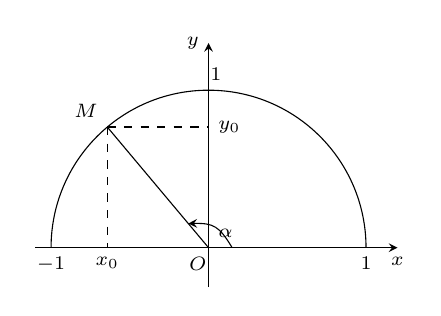
\begin{tikzpicture}[>=stealth,font=\scriptsize]
			\draw[->] (-2.2,0) -- (2.4,0) node[below]{$x$};
			\draw[->] (0,-.5) -- (0,2.6) node[left]{$y$};
			\draw (.1,0) node[below left]{$O$}
			(-2,0) node[below]{$-1$}
			(2,0) node[below]{$1$}
			(-0.1,2) node[above right]{$1$};
			\draw (2,0) arc (0:180:2cm);
			\path (130:2cm) coordinate (M);
			\draw[dashed] (M) node[above left]{$M$} -- (M|- 0,0) node[below]{$x_0$};
			\draw[dashed] (M) -- (M -|0,0) node[right]{$y_0$};
			\draw (0,0) -- (M);
			\draw[->] (0.3,0) to [bend right,looseness=1.3] (130:0.4cm) node[above right,midway]{$\alpha$};
	\end{tikzpicture}}
	\end{gachsoc}
	\item [\iconMT] \indam{Bảng giá trị lượng giác của góc đặc biệt:}
	\begin{center}
		\renewcommand{\arraystretch}{2}
		\begin{tabular}{|c|c|c|c|c|c|c|}
			\hline
		 & $0^\circ$ & $30^\circ$ & $45^\circ$ & $60^\circ$ & $90^\circ$ & $180^\circ$\\
			\hline
			$\sin \alpha$  & $0$ & $\dfrac{1}{2}$ & $\dfrac{\sqrt{2}}{2}$ & $\dfrac{\sqrt{3}}{2}$ & $1$ & $0$\\
			\hline
			$\cos \alpha$  & $1$ & $\dfrac{\sqrt{3}}{2}$ & $\dfrac{\sqrt{2}}{2}$ & $\dfrac{1}{2}$ & $0$ & $-1$\\
			\hline
			$\tan \alpha$ & $0$ & $\dfrac{1}{\sqrt{3}}$ & $1$ & $\sqrt{3}$ & $\big|\big|$ & $0$\\
			\hline
			$\cot \alpha$ & $\big|\big|$ & $\sqrt{3}$ & $1$ & $\dfrac{1}{\sqrt{3}}$ & $0$ & $\big|\big|$\\
			\hline
		\end{tabular}
	\end{center}
\item \indam{Các công thức cơ bản:} 
\begin{tcolorbox}[colframe=orange,colback=white,boxrule=0.2mm]
	\begin{listEX}[3]
		\item [\ding{172}] $\tan \alpha=
		\dfrac{\sin\alpha}{\cos\alpha}$;
		\item [\ding{173}]  $\cot \alpha=
		\dfrac{\cos\alpha}{\sin\alpha}$;
		\item [\ding{174}] $\tan \alpha=\dfrac{1}{\cot\alpha}$;
		\item [\ding{175}] $\sin^2\alpha + \cos^2\alpha =1$;
		\item [\ding{176}] $1+\tan^2\alpha=\dfrac{1}{\cos^2\alpha}$;
		\item [\ding{177}] $1+\cot^2\alpha=\dfrac{1}{\sin^2\alpha}$.
	\end{listEX}
\end{tcolorbox}
\end{itemize}
\subsubsection{Mối quan hệ giữa các giá trị lượng giác}
\begin{itemize}
	\item [\iconMT] \indam{Hai góc bù nhau:} Trên hình bên ta có dây cung $NM$ song song với trục $Ox$ và nếu $\widehat{xOM}=\alpha $ thì $\widehat{xON}=180^\circ-\alpha $. Ta có $y_{M}=y_{N}=y_0,$ $x_{M}=-x_{N}=x_0$. Do đó
	\begin{gachsoc}	
			\immini{
			\begin{listEX}[1]
			\item [\ding{172}] $\sin (180^\circ-\alpha )=\sin \alpha$
			\item [\ding{173}] $\cos (180^\circ-\alpha )=-\cos \alpha$
			\item [\ding{174}] $\tan (180^\circ-\alpha )=-\tan \alpha$
			\item [\ding{175}] $\cot (180^\circ-\alpha )=-\cot \alpha$
		\end{listEX}
	}{\begin{tikzpicture}[scale=1, font=\footnotesize,>=stealth,x=2cm,y=2cm]
			\def\x{0.715}
			\def\a{44}
			\pgfmathsetmacro{\y}{\x*tan(\a)}
			\draw[->] (-1.3,0)--(1.3,0) node [below]{$x$};
			\draw[->] (0,-0.2)--(0,1.3) node [left]{$y$};
			\node at (0,0) [below left]{$O$};
			\draw (1,0) arc (0:180:2cm);
			\fill (1,0) node[below]{$1$} circle(1pt);
			\fill (-1,0) node[below]{$-1$} circle(1pt);
			\fill (0,1) node[above left]{$1$} circle(1pt);
			\fill (\x,0) node[below]{$x_0$} circle(1pt);
			\fill (-\x,0) node[below]{$-x_0$} circle(1pt);
			\fill (\a:1) node[above right]{$M$} circle(1pt);
			\fill (180-\a:1) node[above left]{$N$} circle(1pt);
			\fill (0,\y) node[above right]{$y_0$} circle(1pt);
			\draw[dashed] (\x,0)|-(0,\y);
			\draw[dashed] (-\x,0)|-(0,\y);
			\draw (44:1)--(0,0)--(136:1);
			\draw (0.3,0) arc (0:\a:0.6cm);
			\node at (0,0)[shift={(25:0.2)}]{\tiny{$\alpha$}};
			\draw (0.2,0) coordinate (A) -- (0,0) coordinate (B) -- (136:0.6 cm) coordinate (C) pic [draw, double, angle radius = 9mm] {angle = A--B--C}; 
			\draw (0.25,0.55)node{\tiny{$180^\circ-\alpha$}};
	\end{tikzpicture}}
		\end{gachsoc}
	\item [\iconMT] \indam{Hai góc phụ nhau:} Hình vẽ bên, hai điểm $M$ và $N$ ứng với hai góc phụ nhau $\alpha$ và $90^\circ-\alpha$ ($\widehat{xOM}=\alpha$, $\widehat{xON}=90^\circ-\alpha$ )
	\begin{gachsoc}
		\immini{	\begin{itemize}
				\item [$\bullet$] $\cos \left( 90^\circ-\alpha  \right) = \sin \alpha$
				\item [$\bullet$] $\sin \left(90^\circ-\alpha  \right) = \cos \alpha$
				\item [$\bullet$] $\tan \left(90^\circ-\alpha  \right) = \cot \alpha$
				\item [$\bullet$] $\cot \left( 90^\circ-\alpha  \right) = \tan \alpha$
			\end{itemize}
		}{
			\begin{tikzpicture}[scale=1, font=\footnotesize,>=stealth,x=2cm,y=2cm]
				\def\x{0.866}
				\def\a{30}
				\pgfmathsetmacro{\y}{\x*tan(\a)}
				\draw[->] (-1.3,0)--(1.3,0) node [below]{$x$};
				\draw[->] (0,-0.2)--(0,1.3) node [left]{$y$};
				\node at (0,0) [below left]{$O$};
				\draw (1,0) arc (0:180:2cm);
				\fill (1,0) node[below]{$1$} circle(1pt);
				\fill (-1,0) node[below]{$-1$} circle(1pt);
				\fill (0,1) node[above left]{$1$} circle(1pt);
				\fill (\x,0) node[below]{$x_0$} circle(1pt);
				\fill (\a:1) node[above right]{$M$} circle(1pt);
				\fill (90-\a:1) node[above right]{$N$} circle(1pt);
				\fill (0,\y) node[above left]{$y_0$} circle(1pt);
				\draw[dashed] (\x,0)|-(0,\y);
				\draw[dashed] (\y,0)|-(0,\x);
				\draw (\a:1)--(0,0)--(90-\a:1);
				\draw (0.3,0) arc (0:\a:0.6cm);
				\node at (0,0)[shift={(15:0.25)}]{\tiny{$\alpha$}};
				\draw (0.2,0) coordinate (A) -- (0,0) coordinate (B) -- (90-\a:0.6 cm) coordinate (C) pic [draw, double, angle radius = 9mm] {angle = A--B--C}; 
				\draw (0.55,0.3)node{\tiny{$90^\circ-\alpha$}};
		\end{tikzpicture}}
	\end{gachsoc}
\end{itemize}

\subsection{RÈN LUYỆN KĨ NĂNG GIẢI TOÁN}
\begin{dang}{Giá trị lượng giác của góc $\alpha$ cho trước ($0^\circ\le \alpha \le 180^\circ$)}
\end{dang}
\begin{vd}
	Bằng cách vẽ nửa đường tròn đơn vị, hãy tính các giá trị lượng giác của góc $\alpha$ với
	\begin{enumEX}[a)]{4}
		\item $\alpha = 60^\circ$.
		\item $\alpha = 90^\circ$.
		\item $\alpha = 120^\circ$.
		\item $\alpha = 135^\circ$.
	\end{enumEX}
	\loigiai{
		Trên mặt phẳng tọa độ $Oxy$, nửa đường tròn tâm $O$, bán kính $R = 1$ nằm phía trên trục hoành được gọi là nửa đường tròn đơn vị. Với mỗi góc $\alpha$ ($0^\circ \le \alpha \le 180^\circ$), ta xác định được duy nhất một điểm $M(x_0; y_0)$ trên nửa đường tròn đơn vị sao cho $\widehat{xOM} = \alpha$. Khi đó:
		$$ \sin \alpha = y_0; \quad \cos \alpha = x_0; \quad \tan \alpha = \dfrac{y_0}{x_0} \, (\alpha \neq 90^\circ); \quad \cot \alpha = \dfrac{x_0}{y_0} \, (\alpha \neq 0^\circ, 180^\circ). $$
		
		\begin{center}
			\begin{tikzpicture}[scale=3.5, font=\footnotesize, >=stealth, line join=round, line cap=round]
				% Hệ trục tọa độ
				\draw[->] (-1.3,0) -- (1.3,0) node[below] {$x$};
				\draw[->] (0,-0.2) -- (0,1.3) node[left] {$y$};
				\node[below left] at (0,0) {$O$};
				\draw (1,0) node[below right] {$1$};
				\draw (-1,0) node[below left] {$-1$};
				
				% Nửa đường tròn đơn vị
				\draw[thick, blue] (1,0) arc (0:180:1);
				
				% Điểm M1 cho 60 độ
				\coordinate (M1) at ({cos(60)},{sin(60)});
				\fill (M1) circle (0.8pt) node[above right] {$M_1$};
				\draw[dashed] (M1) -- ({cos(60)},0) node[below] {$\dfrac{1}{2}$};
				\draw[dashed] (M1) -- (0,{sin(60)}) node[right] {$\dfrac{\sqrt{3}}{2}$};
				\draw (0,0) -- (M1);
				\draw[->] (0.2,0) arc (0:60:0.2);
				\node at (0.35, 0.15) {$60^\circ$};
				
				% Điểm M2 cho 90 độ
				\coordinate (M2) at (0,1);
				\fill (M2) circle (0.8pt) node[above right] {$M_2(0; 1)$};
				
				% Điểm M3 cho 120 độ
				\coordinate (M3) at ({cos(120)},{sin(120)});
				\fill (M3) circle (0.8pt) node[above left] {$M_3$};
				\draw[dashed] (M3) -- ({cos(120)},0) node[below] {$-\dfrac{1}{2}$};
				\draw[dashed] (M3) -- (0,{sin(120)});
				\draw (0,0) -- (M3);
				
				% Điểm M4 cho 135 độ
				\coordinate (M4) at ({cos(135)},{sin(135)});
				\fill (M4) circle (0.8pt) node[above left] {$M_4$};
				\draw[dashed] (M4) -- ({cos(135)},0) node[below] {$-\dfrac{\sqrt{2}}{2}$};
				\draw[dashed] (M4) -- (0,{sin(135)}) node[left] {$\dfrac{\sqrt{2}}{2}$};
				\draw (0,0) -- (M4);
			\end{tikzpicture}
		\end{center}
		
		\begin{enumerate}
			\item[a)] Với $\alpha = 60^\circ$, điểm $M_1$ trên nửa đường tròn đơn vị sao cho $\widehat{xOM_1} = 60^\circ$ có tọa độ là $M_1\left(\dfrac{1}{2}; \dfrac{\sqrt{3}}{2}\right)$. Do đó:
			$$ \sin 60^\circ = \dfrac{\sqrt{3}}{2}; \quad \cos 60^\circ = \dfrac{1}{2}; \quad \tan 60^\circ = \sqrt{3}; \quad \cot 60^\circ = \dfrac{\sqrt{3}}{3}. $$
			
			\item[b)] Với $\alpha = 90^\circ$, điểm $M_2$ trên nửa đường tròn đơn vị sao cho $\widehat{xOM_2} = 90^\circ$ chính là giao điểm của nửa đường tròn với phần dương trục $Oy$. Điểm này có tọa độ là $M_2(0; 1)$. Do đó:
			$$ \sin 90^\circ = 1; \quad \cos 90^\circ = 0; \quad \cot 90^\circ = 0. $$
			(Không tồn tại $\tan 90^\circ$).
			
			\item[c)] Với $\alpha = 120^\circ$, điểm $M_3$ trên nửa đường tròn đơn vị sao cho $\widehat{xOM_3} = 120^\circ$ có tọa độ là $M_3\left(-\dfrac{1}{2}; \dfrac{\sqrt{3}}{2}\right)$. Do đó:
			$$ \sin 120^\circ = \dfrac{\sqrt{3}}{2}; \quad \cos 120^\circ = -\dfrac{1}{2}; \quad \tan 120^\circ = -\sqrt{3}; \quad \cot 120^\circ = -\dfrac{\sqrt{3}}{3}. $$
			
			\item[d)] Với $\alpha = 135^\circ$, điểm $M_4$ trên nửa đường tròn đơn vị sao cho $\widehat{xOM_4} = 135^\circ$ có tọa độ là $M_4\left(-\dfrac{\sqrt{2}}{2}; \dfrac{\sqrt{2}}{2}\right)$. Do đó:
			$$ \sin 135^\circ = \dfrac{\sqrt{2}}{2}; \quad \cos 135^\circ = -\dfrac{\sqrt{2}}{2}; \quad \tan 135^\circ = -1; \quad \cot 135^\circ = -1. $$
		\end{enumerate}
	}
\end{vd} \dongcham{15}
	\begin{vd}
		Bằng cách vẽ nửa đường tròn đơn vị, hãy tìm góc $\alpha$ ($0^\circ\le \alpha \le 180^\circ$) trong các trường hợp sau:
		\begin{enumEX}[a)]{4}
			\item $\cos\alpha=-\dfrac{\sqrt{2}}{2}$
			\item $\cos\alpha=\dfrac{1}{2}$
			\item $\sin\alpha=\dfrac{\sqrt{2}}{2}$
			\item $\sin\alpha=1$
		\end{enumEX}
	\loigiai{
		Trên nửa đường tròn đơn vị, mỗi góc $\alpha$ ($0^\circ \le \alpha \le 180^\circ$) tương ứng với duy nhất một điểm $M(x; y)$ sao cho $\widehat{xOM} = \alpha$. Khi đó, hoành độ $x = \cos \alpha$ và tung độ $y = \sin \alpha$.
		
		\begin{center}
			\begin{tikzpicture}[scale=3.5, font=\footnotesize, >=stealth, line join=round, line cap=round]
				% Hệ trục tọa độ
				\draw[->] (-1.3,0) -- (1.3,0) node[below] {$x$};
				\draw[->] (0,-0.2) -- (0,1.3) node[left] {$y$};
				\node[below left] at (0,0) {$O$};
				\draw (1,0) node[below right] {$1$};
				\draw (-1,0) node[below left] {$-1$};
				
				% Nửa đường tròn đơn vị
				\draw[thick, blue] (1,0) arc (0:180:1);
				
				% b) cos = 1/2 -> 60 độ
				\coordinate (M1) at ({cos(60)},{sin(60)});
				\fill (M1) circle (0.8pt) node[above right] {$M_1$};
				\draw[dashed] ({cos(60)},0) node[below] {$\dfrac{1}{2}$} -- (M1);
				\draw (0,0) -- (M1);
				
				% c) sin = sqrt(2)/2 -> 45 độ và 135 độ
				\coordinate (M2) at ({cos(45)},{sin(45)});
				\fill (M2) circle (0.8pt) node[above right] {$M_2$};
				\draw[dashed] ({cos(45)},0) node[below] {$\dfrac{\sqrt{2}}{2}$} -- (M2) -- (0,{sin(45)}) node[right] {$\dfrac{\sqrt{2}}{2}$};
				\draw (0,0) -- (M2);
				
				% a) cos = -sqrt(2)/2 -> 135 độ
				\coordinate (M3) at ({cos(135)},{sin(135)});
				\fill (M3) circle (0.8pt) node[above left] {$M_3$};
				\draw[dashed] ({cos(135)},0) node[below] {$-\dfrac{\sqrt{2}}{2}$} -- (M3) -- (0,{sin(135)});
				\draw (0,0) -- (M3);
				
				% Kẻ đường nối M2 và M3 (cùng tung độ)
				\draw[dashed] (M3) -- (M2);
				
				% d) sin = 1 -> 90 độ
				\coordinate (M4) at (0,1);
				\fill (M4) circle (0.8pt) node[above right] {$M_4(0; 1)$};
			\end{tikzpicture}
		\end{center}
		
		\begin{enumerate}
			\item[a)] Tìm điểm $M$ trên nửa đường tròn có hoành độ $x = -\dfrac{\sqrt{2}}{2}$. Qua điểm $-\dfrac{\sqrt{2}}{2}$ trên trục $Ox$, kẻ đường thẳng vuông góc với trục hoành cắt nửa đường tròn tại $M_3$. Điểm $M_3$ tương ứng với góc $\alpha = 135^\circ$. Vậy $\alpha = 135^\circ$.
			
			\item[b)] Tìm điểm $M$ trên nửa đường tròn có hoành độ $x = \dfrac{1}{2}$. Qua điểm $\dfrac{1}{2}$ trên trục $Ox$, kẻ đường thẳng vuông góc với trục hoành cắt nửa đường tròn tại $M_1$. Điểm $M_1$ tương ứng với góc $\alpha = 60^\circ$. Vậy $\alpha = 60^\circ$.
			
			\item[c)] Tìm điểm $M$ trên nửa đường tròn có tung độ $y = \dfrac{\sqrt{2}}{2}$. Qua điểm $\dfrac{\sqrt{2}}{2}$ trên trục $Oy$, kẻ đường thẳng vuông góc với trục tung cắt nửa đường tròn tại hai điểm $M_2$ và $M_3$. 
			\begin{itemize}
				\item Điểm $M_2$ (thuộc góc phần tư thứ nhất) tương ứng với $\alpha = 45^\circ$.
				\item Điểm $M_3$ (thuộc góc phần tư thứ hai) tương ứng với $\alpha = 135^\circ$.
			\end{itemize}
			Vậy có hai giá trị thỏa mãn: $\alpha = 45^\circ$ hoặc $\alpha = 135^\circ$.
			
			\item[d)] Tìm điểm $M$ trên nửa đường tròn có tung độ $y = 1$. Điểm duy nhất thỏa mãn là điểm $M_4(0; 1)$ nằm trên trục tung, tương ứng với góc $\alpha = 90^\circ$. Vậy $\alpha = 90^\circ$.
		\end{enumerate}
	}
	\end{vd} \dongcham{22}
\begin{vd}
	Trên mặt phẳng toạ độ $Oxy$, lấy điểm $M$ thuộc nửa đường tròn đơn vị sao cho $\widehat{xOM}=120^{\circ}$. Gọi $N$ là điểm đối xứng với $M$ qua trục tung. Tính giá trị của $\tan\widehat{xON}$.
	\loigiai{
	Ta có $\widehat{xOM}$ và $\widehat{xON}$ là hai góc bù nhau nên $\widehat{xON}=180^\circ-120^\circ=60^\circ$.\\
	Suy ra $\tan\widehat{xON}=\tan 60^\circ =\sqrt{3}$.
	}
\end{vd} \dongcham{12}
\begin{dang}{Tính giá trị biểu thức}
\end{dang}

\begin{vd}%[0H2Y1]
	Tính giá trị biểu thức sau
	\begin{tasks}(2)
		\task $A= 2\cos 30^\circ+3\sin 120^\circ$.
		\task $B=a\cdot\cos60^{\circ}+2a\tan45^{\circ}-3a\sin30^{\circ}$.
	\end{tasks}
	\loigiai{
		\begin{enumerate}
			\item[a)] Thay các giá trị lượng giác của các góc đặc biệt vào biểu thức, ta có:
			\begin{align*}
				A &= 2 \cos 30^\circ + 3 \sin 120^\circ \\
				&= 2 \cdot \dfrac{\sqrt{3}}{2} + 3 \cdot \dfrac{\sqrt{3}}{2} \\
				&= \sqrt{3} + \dfrac{3\sqrt{3}}{2} \\
				&= \dfrac{2\sqrt{3} + 3\sqrt{3}}{2} \\
				&= \dfrac{5\sqrt{3}}{2}.
			\end{align*}
			Vậy $A = \dfrac{5\sqrt{3}}{2}$.
			
			\item[b)] Tương tự, thay các giá trị lượng giác vào biểu thức, ta có:
			\begin{align*}
				B &= a \cdot \cos 60^\circ + 2a \tan 45^\circ - 3a \sin 30^\circ \\
				&= a \cdot \dfrac{1}{2} + 2a \cdot 1 - 3a \cdot \dfrac{1}{2} \\
				&= \dfrac{a}{2} + 2a - \dfrac{3a}{2} \\
				&= 2a - \left( \dfrac{3a}{2} - \dfrac{a}{2} \right) \\
				&= 2a - \dfrac{2a}{2} \\
				&= 2a - a = a.
			\end{align*}
			Vậy $B = a$.
		\end{enumerate}
		
	}
\end{vd} \dongcham{3}

\begin{vd}
	Biết $\sin15^\circ=\dfrac{\sqrt{3}-1}{2\sqrt{2}}$. Tính giá trị biểu thức 
	\begin{tasks}(2)
		\task $P=\sin165^\circ+\cos75^\circ$.
		\task $Q=\cos165^\circ+\cos75^\circ$.
	\end{tasks}
	\loigiai{
		\begin{enumEX}[a)]{1}
			\item Ta có 
			\begin{itemize}
				\item [$\bullet$] $\sin165^\circ = \sin (180^\circ - 165^\circ)=\sin 15^\circ$;
				\item [$\bullet$] $\cos 75^\circ =\sin(90^\circ -75^\circ)=\sin 15^\circ$ 
			\end{itemize}
			Suy ra
			$$P=\sin165^\circ+\cos75^\circ=2\sin 15^\circ=2\dfrac{\sqrt{3}-1}{2\sqrt{2}}=\dfrac{\sqrt{3}-1}{\sqrt{2}}$$
			\item Ta có 
			\begin{itemize}
				\item [$\bullet$] $\cos165^\circ = \cos (180^\circ - 165^\circ)=-\cos 15^\circ$;
				\item [$\bullet$] $\cos 75^\circ =\sin(90^\circ -75^\circ)=\sin 15^\circ$ 
			\end{itemize}
			Suy ra
			$$P=\sin 15^\circ-\cos 15^\circ=\sin 15^\circ-\sqrt{\sin 15^\circ}=\dfrac{\sqrt{3}-1}{\sqrt{2}}=\dfrac{6}{2}.$$
		\end{enumEX}
		
	}
\end{vd} \dongcham{6}

\begin{vd}%[Tex hóa SGK CD-CT,T7/22, Cao Thành Thái]%[0H2K1-3]
	Tính giá trị đúng của các biểu thức sau (không dùng máy tính cầm tay).
	\begin{enumEX}[a)]{1}
		\item $A=\cos 0^\circ + \cos 40^\circ + \cos 120^\circ + \cos 140^\circ$;
		\item $B=\sin 5^\circ + \sin 150^\circ - \sin 175^\circ + \sin 180^\circ$;
		\item $C=\cos 15^\circ + \cos 35^\circ - \sin 75^\circ - \sin 55^\circ$;
		\item $D=\tan 25^\circ\cdot \tan 45^\circ\cdot \tan 115^\circ$.
	\end{enumEX}
	\loigiai
	{
		\begin{enumerate}
			\item $\begin{aligned}[t]
				A &=\cos 0^\circ + \cos 40^\circ + \cos 120^\circ + \cos 140^\circ \\
				&= \cos 0^\circ + \cos 40^\circ + \cos\left(180^\circ - 60^\circ\right) + \cos\left(180^\circ - 40^\circ\right)\\
				&=\cos 0^\circ + \cos 40^\circ - \cos 60^\circ - \cos 40^\circ = \cos 0^\circ - \cos 60^\circ = 1-\dfrac{1}{2} = \dfrac{1}{2}.
			\end{aligned}$
			\item $\begin{aligned}[t]
				B &=\sin 5^\circ + \sin 150^\circ - \sin 175^\circ + \sin 180^\circ \\
				&= \sin 5^\circ + \sin\left(180^\circ-30^\circ\right) - \sin\left(180^\circ-5^\circ\right) + \sin 180^\circ\\
				&=\sin 5^\circ + \sin 30^\circ - \sin 5^\circ + \sin 180^\circ = \sin 30^\circ + \sin 180^\circ = \dfrac{1}{2}+0 = \dfrac{1}{2}.
			\end{aligned}$
			\item $\begin{aligned}[t]
				C &=\cos 15^\circ + \cos 35^\circ - \sin 75^\circ - \sin 55^\circ = \cos 15^\circ + \cos 35^\circ - \sin\left(90^\circ-15^\circ\right) - \sin\left(90^\circ-35^\circ\right)\\
				&=\cos 15^\circ + \cos 35^\circ - \cos 15^\circ - \cos 35^\circ = 0.
			\end{aligned}$
			\item $\begin{aligned}[t]
				D &=\tan 25^\circ\cdot \tan 45^\circ\cdot \tan 115^\circ = \tan 25^\circ\cdot \tan 45^\circ\cdot \tan\left(180^\circ - 65^\circ\right)\\
				&= \tan 25^\circ\cdot \tan 45^\circ\cdot \left(-\tan 65^\circ\right)=-\tan 25^\circ\cdot \tan 45^\circ\cdot  \tan 65^\circ \\
				&=-\tan 25^\circ\cdot \tan 45^\circ\cdot \tan\left(90^\circ - 25^\circ\right) = -\tan 25^\circ\cdot \tan 45^\circ\cdot \cot 25^\circ\\
				&=-\left(\tan 25^\circ \cdot \cot 25^\circ\right)\tan 45^\circ = -1\cdot 1 = -1.
			\end{aligned}$
		\end{enumerate}
	}
\end{vd}
\dongcham{16}
\begin{dang}{Rút gọn, chứng minh biểu thức}
\end{dang}

\begin{vd}
	Tính các giá trị lượng giác còn lại của góc $\alpha $, biết
	\begin{tasks}(2)
		\task $\sin \alpha =\dfrac{1}{3}$ và $90^{\circ}<\alpha <180^{\circ}$;
		\task $\cos \alpha =\dfrac{3}{5}$ và $0^\circ <\alpha <90^\circ$;
		\task $\tan \alpha =\sqrt{3}$ và $0^\circ <\alpha <90^\circ$;
		\task $\tan \alpha =3$ và $90^{\circ}<\alpha <180^{\circ}$.
	\end{tasks}
	\loigiai{
		\begin{enumerate}[a)]
			\item Ta có $\cos^2 \alpha=1-\sin^2\alpha = 1-\dfrac{1}{9}=\dfrac{8}{9} \Rightarrow \cos \alpha = \pm \dfrac{2\sqrt{2}}{3}$.\\
			Do $90^{\circ}<\alpha <180^{\circ}$ nên $\cos \alpha <0$, suy ra $\cos \alpha = - \dfrac{2\sqrt{2}}{3}$
			\begin{itemize}
				\item  $\tan \alpha = \dfrac{\sin \alpha}{\cos \alpha}=-\dfrac{1}{2\sqrt{2}}$.
				\item  $\cot \alpha = \dfrac{1}{\tan \alpha}=-2\sqrt{2}$.
			\end{itemize} 
			\item Ta có $\sin^2 \alpha=1-\cos^2\alpha = 1-\dfrac{9}{25}=\dfrac{16}{25} \Rightarrow \sin \alpha = \pm \dfrac{4}{5}$.\\
			Do $0^\circ <\alpha <90^\circ$ nên $\sin \alpha >0$, suy ra $\sin \alpha = \dfrac{4}{5}$
			\begin{itemize}
				\item  $\tan \alpha = \dfrac{\sin \alpha}{\cos \alpha}=\dfrac{3}{4}$.
				\item  $\cot \alpha = \dfrac{1}{\tan \alpha}=\dfrac{4}{3}$.
			\end{itemize} 
		\item Ta có $\cos^2 \alpha=\dfrac{1}{1+\tan^2 \alpha}= \dfrac{1}{4} \Rightarrow \cos \alpha =\pm \dfrac{1}{2}$.\\
		Do $0^\circ <\alpha <90^\circ$ nên $\cos \alpha >0$, suy ra $\cos \alpha =  \dfrac{1}{2}$.
		\begin{itemize}
			\item  $\tan \alpha = \dfrac{\sin \alpha}{\cos \alpha} \Rightarrow \sin \alpha = \tan \alpha \cdot \cos \alpha =  \dfrac{\sqrt{3}}{2}$.
			\item  $\cot \alpha = \dfrac{1}{\tan \alpha}=\dfrac{1}{\sqrt{3}}$.
		\end{itemize} 
		\item Ta có $\cos^2 \alpha=\dfrac{1}{1+\tan^2 \alpha}= \dfrac{1}{10} \Rightarrow \cos \alpha =\pm \dfrac{\sqrt{10}}{10}$.\\
		Do $90^{\circ}<\alpha <180^{\circ}$ nên $\cos \alpha <0$, suy ra $\cos \alpha = - \dfrac{\sqrt{10}}{10}$.
		\begin{itemize}
			\item  $\tan \alpha = \dfrac{\sin \alpha}{\cos \alpha} \Rightarrow \sin \alpha = \tan \alpha \cdot \cos \alpha = - \dfrac{3\sqrt{10}}{10}$.
			\item  $\cot \alpha = \dfrac{1}{\tan \alpha}=- \dfrac{\sqrt{10}}{3}$.
		\end{itemize}
	\end{enumerate}}
\end{vd}
\dongcham{18}
\begin{vd}
	Cho góc $x$ với $\cos x = -\dfrac{1}{2}$. Tính giá trị của biểu thức $S = 4\sin^2 x + 8\tan^2 x$.
	\loigiai{
		Áp dụng các hằng đẳng thức lượng giác cơ bản, ta có:
		\begin{itemize}
			\item $\sin^2 x = 1 - \cos^2 x = 1 - \left(-\dfrac{1}{2}\right)^2 = 1 - \dfrac{1}{4} = \dfrac{3}{4}$.
			\item $\tan^2 x = \dfrac{\sin^2 x}{\cos^2 x} = \dfrac{\dfrac{3}{4}}{\left(-\dfrac{1}{2}\right)^2} = \dfrac{\dfrac{3}{4}}{\dfrac{1}{4}} = 3$.
		\end{itemize}
		
		Thay các giá trị vừa tính được vào biểu thức $S$, ta được:
		$$ S = 4 \cdot \dfrac{3}{4} + 8 \cdot 3 = 3 + 24 = 27. $$
		
		Vậy $S = 27$.
	}
\end{vd}
\dongcham{4}
\begin{vd}
	Cho $90^\circ < \alpha < 180^\circ$, $0^\circ < \beta < 90^\circ$ và $\alpha - \beta = 90^\circ$. Chứng minh:
	\begin{enumEX}[a)]{3}
		\item $\sin\alpha = \cos\beta$;
		\item $\cos\alpha = -\sin\beta$;
		\item $\tan\alpha = -\cot\beta$.
	\end{enumEX}
	\loigiai{
		Từ giả thiết $\alpha - \beta = 90^\circ$, ta suy ra $\alpha = 90^\circ + \beta$.
		
		Xét góc bù của góc $\alpha$ là góc $180^\circ - \alpha$. Thay $\alpha = 90^\circ + \beta$ vào biểu thức, ta được:
		$$ 180^\circ - \alpha = 180^\circ - (90^\circ + \beta) = 90^\circ - \beta. $$
		Như vậy, hai góc $180^\circ - \alpha$ và $\beta$ là hai góc phụ nhau (có tổng số đo bằng $90^\circ$).
		
		Áp dụng tính chất giá trị lượng giác của hai góc phụ nhau và hai góc bù nhau, ta có:
		\begin{enumerate}
			\item[a)] Vì $180^\circ - \alpha$ và $\beta$ là hai góc phụ nhau nên:
			$$ \sin(180^\circ - \alpha) = \cos\beta $$
			Mặt khác, vì $\alpha$ và $180^\circ - \alpha$ là hai góc bù nhau nên $\sin(180^\circ - \alpha) = \sin\alpha$.
			Từ đó suy ra: $\sin\alpha = \cos\beta$ (điều phải chứng minh).
			
			\item[b)] Tương tự, vì $180^\circ - \alpha$ và $\beta$ phụ nhau nên:
			$$ \cos(180^\circ - \alpha) = \sin\beta $$
			Mặt khác, $\cos(180^\circ - \alpha) = -\cos\alpha$ (tính chất hai góc bù nhau).
			Suy ra: $-\cos\alpha = \sin\beta \Leftrightarrow \cos\alpha = -\sin\beta$ (điều phải chứng minh).
			
			\item[c)] Ta có:
			$$ \tan(180^\circ - \alpha) = \cot\beta $$
			Mà $\tan(180^\circ - \alpha) = -\tan\alpha$ (tính chất hai góc bù nhau).
			Suy ra: $-\tan\alpha = \cot\beta \Leftrightarrow \tan\alpha = -\cot\beta$ (điều phải chứng minh).
		\end{enumerate}
		}
\end{vd}
\dongcham{6}
\begin{vd}%[0H2B1]
	Cho $A, B, C$ là các góc của tam giác. Chứng minh các đẳng thức sau:
	\begin{tasks}(2)
		\task $\sin\left(A+B\right)=\sin C.$
		\task $\cos\left(A+B\right)+\cos C=0.$
		\task $\sin\dfrac{A+B}{2}=\cos\dfrac{C}{2}.$
		\task $\tan\left(A-B+C\right)=-\tan2B.$
	\end{tasks}
	\loigiai{ Do $A, B, C$ là các góc của tam giác nên ta có $A+B+C=180^{\circ}$.
		\begin{enumerate}[a)]
			\item Ta có $A+B+C=180^{\circ}\Leftrightarrow A+B=180^{\circ}-C.$\\
			Từ đó suy ra $\sin\left(A+B\right)=\sin \left(180^{\circ}-C\right)=\sin C.$
			\item Ta có $A+B+C=180^{\circ}\Leftrightarrow A+B=180^{\circ}-C.$\\
			Từ đó suy ra $\cos\left(A+B\right)=\cos \left(180^{\circ}-C\right)=-\cos C \Rightarrow \cos\left(A+B\right)+\cos C=0.$
			\item Ta có $A+B+C=180^{\circ}\Leftrightarrow \dfrac{A+B}{2}=\dfrac{180^{\circ}-C}{2}=90^{\circ}-\dfrac{C}{2}.$\\
			Từ đó suy ra $\sin\dfrac{A+B}{2}=\sin\left(90^{\circ}-\dfrac{C}{2}\right)= \cos\dfrac{C}{2}.$
			\item Ta có $\tan\left(A-B+C\right)=\tan\left(A+B+C-2B\right)=\tan\left(180^{\circ}-2B\right)=-\tan2B.$
		\end{enumerate}
	}
	\end{vd} \dongcham{13}